%%%%%%%%%%%%%%%%%%%%%%%%%%%%%%%%%%%%%%%%%%%%%%%%%%%%%%%%%%%%%%%%%%%%%%%%%%%%%%%%
%% 实验报告模板.tex                                                           %%
%% author: hxp<hxp201406@gmail.com>                                           %%
%% 按照基础物理实验老师发的模板更改形成                                       %%
%%%%%%%%%%%%%%%%%%%%%%%%%%%%%%%%%%%%%%%%%%%%%%%%%%%%%%%%%%%%%%%%%%%%%%%%%%%%%%%%
%% 备注:刚刚的注释刚好是80行,编写代码的时候不要超过80行,就是你的代码不要超 %%
%% 过我注释里面最后面的“%”,超过请换行。                                      %%
%%%%%%%%%%%%%%%%%%%%%%%%%%%%%%%%%%%%%%%%%%%%%%%%%%%%%%%%%%%%%%%%%%%%%%%%%%%%%%%%
%% 模板现在开始,请根据注释把相应的位置更改成对应的内容                       %%
%%%%%%%%%%%%%%%%%%%%%%%%%%%%%%%%%%%%%%%%%%%%%%%%%%%%%%%%%%%%%%%%%%%%%%%%%%%%%%%%


\documentclass{ctexart}


\usepackage{ctex}
\usepackage{amsmath}
\usepackage{amsfonts}
\usepackage{amssymb}
\usepackage{wasysym}
\newcommand{\angstrom}{\text{\normalfont\AA}}  % 定义了原子物理的A
\usepackage{graphicx}
\usepackage{float}
\usepackage{geometry}
\geometry{a4paper,scale=0.8}  % 定义页面大小是A4,缩放是0.8
\usepackage{caption}
\usepackage{subcaption}
\usepackage{enumitem}

\newcommand*{\md}{\mathop{}\!\mathrm{d}}   % 定义微分算子,直立体的d
\newcommand*{\me}{\mathrm{e}}              % 定义自然对数e,同样应当是直立体

% 如果你想要每一段的开头不要空两格,注释掉下面这两行
% \usepackage{parskip}
% \setlength{\parindent}{0cm}

% 默认的\mathbf对希腊字母不生效,这里改下
\usepackage{bm}
\let\Oldmathbf\mathbf
\renewcommand{\mathbf}[1]{\boldsymbol{\Oldmathbf{#1}}}

% 表格默认格内内容和边框没有留出距离,显示分数的时候,分数的上下会贴到边框上
% 因此我增加了表格内容和边框的最短距离是5像素
\usepackage{cellspace}
\setlength{\cellspacetoplimit}{5pt}
\setlength{\cellspacebottomlimit}{5pt}

% \si命令是用来写单位的,单位需要和之前的数字有一个空格的距离,而且应当直立体
% 用法:5 \si{km/h}
\newcommand{\si}[1]{\  \mathrm{#1}}

% 日期不要显示
\date{}

\usepackage{fancyhdr}
\pagestyle{fancy}
\fancyhf{}
\lhead{本文档TeX源码地址:https://github.com/hxp-plus/Notes/tree/master/Physics-Experiment/实验报告}
\rfoot{第 \thepage 页}
\renewcommand{\headrulewidth}{1pt}
\renewcommand{\footrulewidth}{1pt}

%% 标题三号黑体,作者信息为班级姓名学号
\newcommand{\generatetitle}[6]{\title{\zihao{3}\heiti#1} \author{#2 \quad
    \quad #3 \quad\quad #4 \quad\quad #5 \quad\quad #6} \maketitle\thispagestyle{fancy}}

%% 所有的引言、实验内容与数据处理啥的,用section
\ctexset {
  section = {
    format = \raggedright\zihao{4}\heiti,  % 设置所有section的字号为四号黑体左对齐
    name={,、},                            % 序号后跟顿号
    aftername={\hspace{0pt}},              % 修改序号和标题直接的间距为零
    number=\chinese{section},              % 设置序号为中文
  },
  subsection = {
    format = \raggedright\zihao{5}\heiti,  % 设置所有subsection的字号为五号黑体左对齐
    number={},              % 设置序号为没有序号
  }
}

%% 实验背景、实验目的啥的,用subsection
\ctexset {
  subsection = {
    format = \raggedright\zihao{5}\heiti,  % 所有subsection的字号为五号黑体左对齐
    number={},                             % 设置序号为没有序号
  }
}

%% 把subsection之间加上中括号
\let\oldsubsection\subsection
\renewcommand{\subsection}[1]{\oldsubsection{\!\!\!\!\!\!【#1】}}

%% 摘要和关键词用paragraph

\ctexset {
  paragraph = {
    format = \raggedright\zihao{5}\heiti,  % 所有paragraph的字号为五号黑体左对齐
    number={},                             % 设置序号为没有序号
  }
}

%% 把paragraph之间加上中括号
\let\oldparagraph\paragraph
\renewcommand{\paragraph}[1]{\oldparagraph{#1:\!\!\!\!\!\!}}

%% 再把参考文献的序号去掉
\makeatletter
\renewcommand\@biblabel[1]{}
\makeatother

\begin{document}

\generatetitle{近代物理实验报告——
  晶体的电光调制}{物理4+4}{胡喜平}{U201811966}{hxp201406@gmail.com}{https://hxp.plus/}

\paragraph{摘要}
电光调制是一种把电信号转化成光信号的技术,通过把电信号转化成光信号,这就可以让原本的电信号通过光纤发射出去,实现光纤通讯。本次实验中我们搭建晶体横向电光调制装置,并输入正弦信号,企图将正弦的电信号转化为光信号,并探索什么条件下信号不会发生失真。

% 关键词
\paragraph{关键词}
电光调制、电光晶体

\section{引言}
\subsection{实验目的}
搭建晶体横向电光调制装置,之后输入正弦电信号,探究什么条件下电信号转化得到的光信号不发生失真,以及什么条件下会发生什么样子的失真。

\section{实验内容与数据处理}
\subsection{实验原理}

下图是晶体横向电光调制装置图,入射光经过起偏器成为平行于x轴的线偏振光,通过电光晶体,$x$分量和$y$分量产生相位差$\delta_1$,通过1/4波片再产生相位差$\delta_2$,最终从平行于$y$轴的检偏器出射。

\begin{figure}[H]
  \centering
  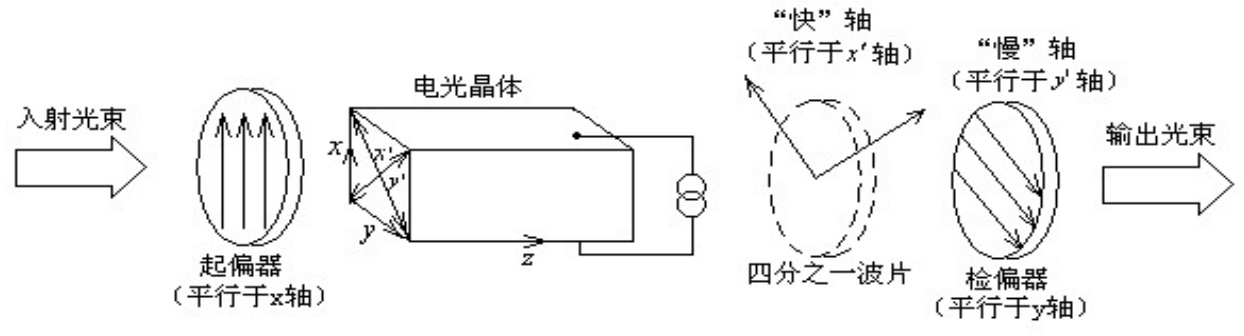
\includegraphics[width=0.9\linewidth]{figures/晶体的横向电光调制}
  \caption{晶体的横向电光调制装置图}
\end{figure}

其中光通过电光晶体产生的相位差$\delta_1$是正比于电光晶体上加的电压的,为

\begin{equation*}
  \begin{aligned}
    \delta = \dfrac{2 \pi}{\lambda} n_0^3 \gamma_{22} V \dfrac{\lambda}{d}  
  \end{aligned}
\end{equation*}

同时,光透过检偏器后透射率为

\begin{equation*}
  \begin{aligned}
    T = \sin^2 \dfrac{\delta_1 + \delta_2}{2} 
  \end{aligned}
\end{equation*}

当晶体两端电压在某一个特定数值的时候,光透过晶体产生$\pi$的相位差,定义这个电压为$V_{\pi}$,则

\begin{equation*}
  \begin{aligned}
    V_{\pi} = \dfrac{\lambda}{2 n_0^3 \gamma_{22}} \left( \dfrac{d}{l}  \right)  
  \end{aligned}
\end{equation*}

则

\begin{equation*}
  \begin{aligned}
    \delta_1 = \pi \dfrac{V}{V_{\pi}} 
  \end{aligned}
\end{equation*}

而本次实验需要运用两个电光调制原理,首先是通过改变直流偏压。

如果我们把直流偏压$V_0$和交流调制信号$V_m \sin \omega t$同时加到电光晶体两端,随着交流调制信号的改变,透过率也会改变。

\begin{equation*}
  \begin{aligned}
    T = \sin^2 \dfrac{\delta_1}{2} = \sin^2 \dfrac{\pi}{2 V_{\pi}} \left( V_0 + V_m \sin \omega t \right)  
  \end{aligned}
\end{equation*}

调制信号不失真应当有两个前提:$V_0$设置的静态工作点处,透射率对于晶体两端电压的偏导数是$1$,且$V_m \ll V_0$。原因看下面的图自然很容易就明白。

\begin{figure}[H]
  \centering
  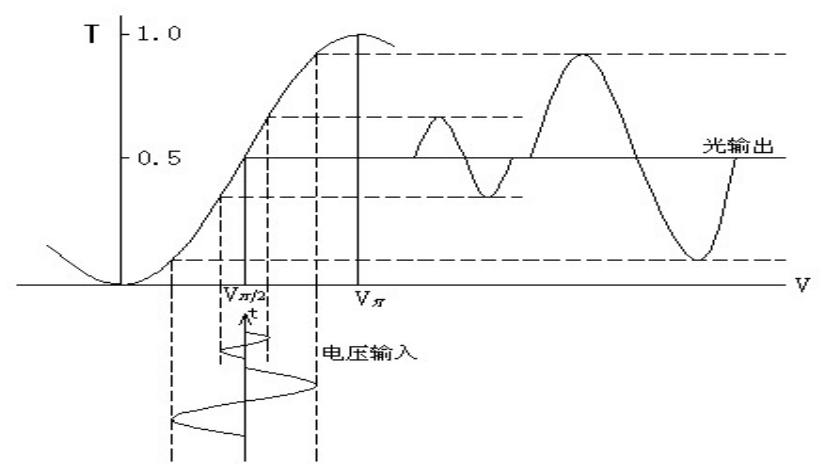
\includegraphics[width=0.7\linewidth]{figures/电光调制原理}
  \caption{电光调制原理图}
\end{figure}

理想的静态工作点是$V_{\pi} / 2$。当$V_0 = V_{\pi} / 2$时,如果有$V_m \ll V_0$,则

\begin{equation*}
  \begin{aligned}
    T \approx \dfrac{1}{2} \left[ 1 + \left( \dfrac{\pi V_m}{V_{\pi}}  \right) \sin \omega t \right]  
  \end{aligned}
\end{equation*}

此时输出波形是我们想要的\textbf{线性调制}信号。

当不满足$V_m \ll V_{\pi}$时,调制信号幅度过大,会出现奇次谐波,输出波形会出现严重\textbf{非线性失真}。

当选择静态工作点$V_0 = V_\pi$或者$V_0 = 0$时,

\begin{equation*}
  \begin{aligned}
    T \approx \dfrac{1}{8} \left( \dfrac{\pi V_m}{V_\pi}  \right)^2 \left( 1 - \cos 2 \omega t \right) 
  \end{aligned}
\end{equation*}

看上面的原理图很容易明白,由于电压高于静态工作点和低于静态工作点时,输出对称的重复图像,所以输出频率是原先的两倍。这种现象称作\textbf{倍频失真}。

除了通过改变直流偏压来进行电光调制,我们也可以通过旋转1/4波片。

我们已经知道影响最后投射光强的本质因素是相位差$\delta_1 + \delta_2$(\textbf{依靠改变直流偏压的电光调制}中没有1/4波片,$\delta_2 = 0$),因此我们除了可以调节晶体两端直流偏置电压$V_0$来改变$\delta_1$来改变最终信号光的相位差,也可以通过更改1/4波片的朝向,来改变$\delta_2$,达成相同的目的。

当1/4波片主轴和检偏器光轴夹角为$0$或者$\pi/2$时,$\delta_2 = 0$,和\textbf{依靠改变直流偏压的电光调制}中设置$V_0 = 0$或者$V_0 = V_{\pi}$是一样的,都会输出\textbf{倍频失真}的波形。

当1/4波片主轴和检偏器光轴夹角为$\pi/4$或者$3\pi/4$时,$\delta_2 = \pi/2$,和\textbf{依靠改变直流偏压的电光调制}中设置$V_0 = V_{\pi}/2$是一样的,输出\textbf{线性调制}的波形。
\subsection{实验内容}

\begin{itemize}
\item 观察电光效应,测量晶体的\textbf{半波电压}。
\item 改变晶体的工作点,观察\textbf{线性调制}、\textbf{倍频失真}、\textbf{非线性调制}。
\item 用1/4波片改变工作点,观察晶体的\textbf{倍频失真}和\textbf{线性调制}。
\end{itemize}

\subsection{实验结果的分析和结论}


调好两个偏振片和电光晶体光轴的方向,先不放偏振片,只加入直流电压,不断调整电压的值,测得输入直流电压为484V时,示波器测得绝对值最大电压,输入直流电压为289V时,示波器测得绝对值最小电压。

\begin{figure}[H]
  \centering
  \begin{subfigure}{.48\textwidth}
    \centering
    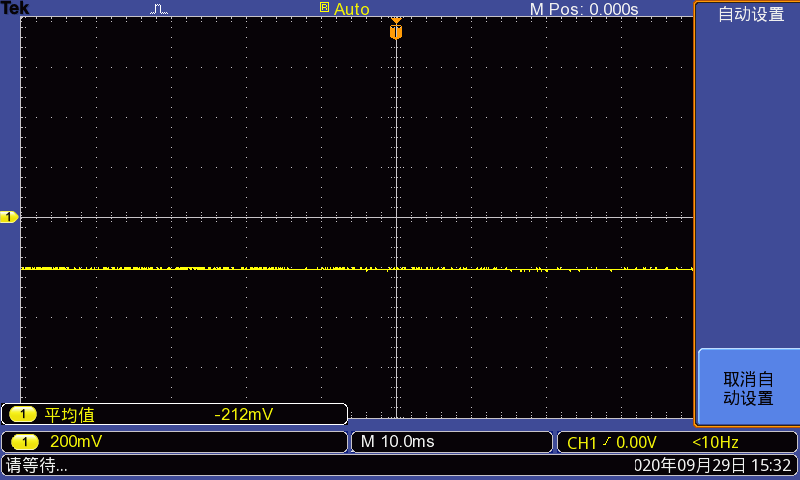
\includegraphics[width=\linewidth]{晶体电光调制图像/没有波片/最大484V/F0001TEK}
    \caption{示波器测得绝对值最大电压}
  \end{subfigure}
  \begin{subfigure}{.48\textwidth}
    \centering
    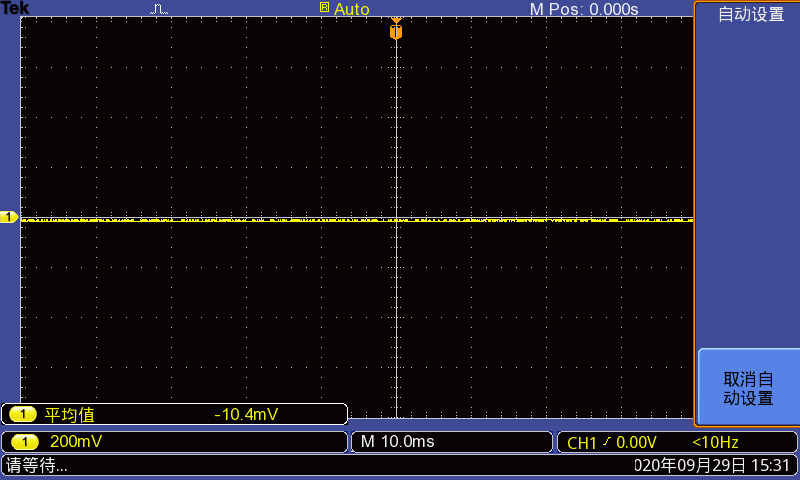
\includegraphics[width=\linewidth]{晶体电光调制图像/没有波片/最小289V/F0000TEK}
    \caption{示波器测得绝对值最小电压}
  \end{subfigure}
  \caption{直流偏置电压的测定}
\end{figure}

而且这个示波器测量的电压会随直流电压周期性改变,因此晶体的半波电压为$484 \si{V} - 289 \si{V} = 195 \si{V}$。而且我们知道了如果直流电压在$484 \si{V}$或者$289 \si{V}$,那输入交流信号,会发生倍频失真。如果直流电压在$484 \si{V}$或者$289 \si{V}$的正中间,即$386.5 \si{V}$,会输出正常不失真的信号。

于是我们加入交流电压信号,调节直流信号,发现电压为$265 \si{V}$时,信号发生倍频失真,电压在$374 \si{V}$时,信号刚好不发生失真。

\begin{figure}[H]
  \centering
  \begin{subfigure}{.48\textwidth}
    \centering
    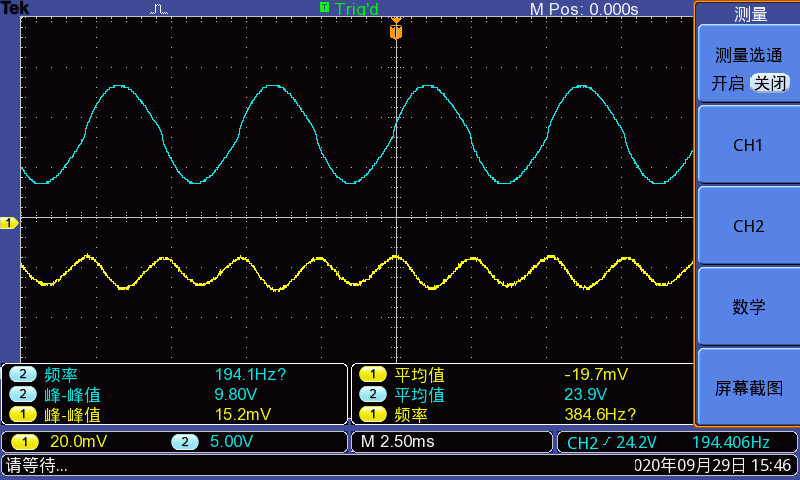
\includegraphics[width=\linewidth]{晶体电光调制图像/没有波片/倍频失真265V/F0000TEK}
    \caption{直流电压265V,倍频失真}
  \end{subfigure}
  \begin{subfigure}{.48\textwidth}
    \centering
    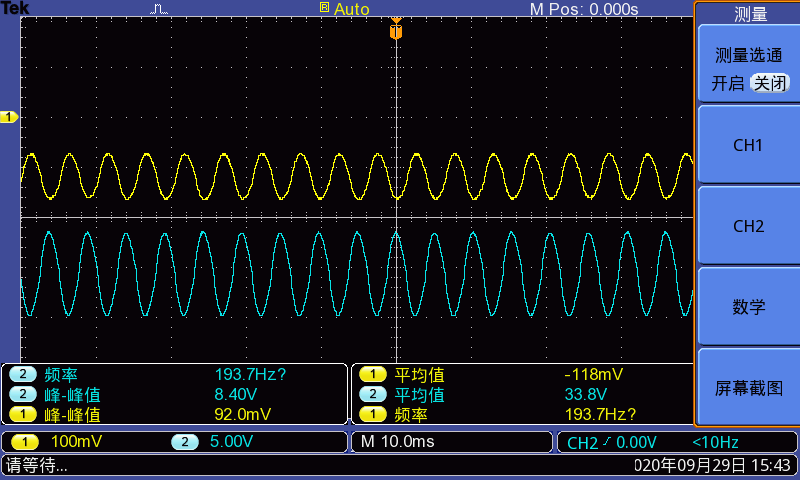
\includegraphics[width=\linewidth]{晶体电光调制图像/没有波片/正弦信号输入偏置374V/F0001TEK}
    \caption{直流电压374V,不失真}
  \end{subfigure}
  \caption{倍频失真和不失真信号的观察}
\end{figure}

然而只要电压稍微偏离一点,就会发生非线性失真,实验中测量了两组非线性失真,直流偏置电压分别为$303 \si{V}$和$440 \si{V}$

\begin{figure}[H]
  \centering
  \begin{subfigure}{.48\textwidth}
    \centering
    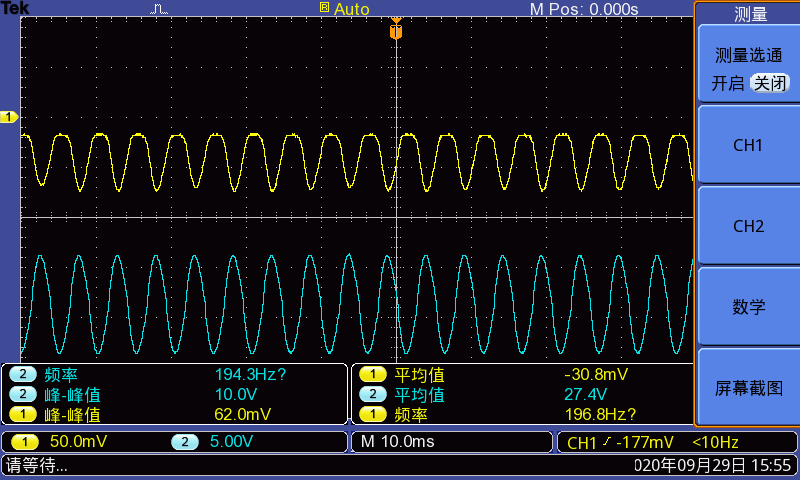
\includegraphics[width=\linewidth]{晶体电光调制图像/没有波片/非线性失真303V/F0000TEK}
    \caption{直流电压303V,上失真}
  \end{subfigure}
  \begin{subfigure}{.48\textwidth}
    \centering
    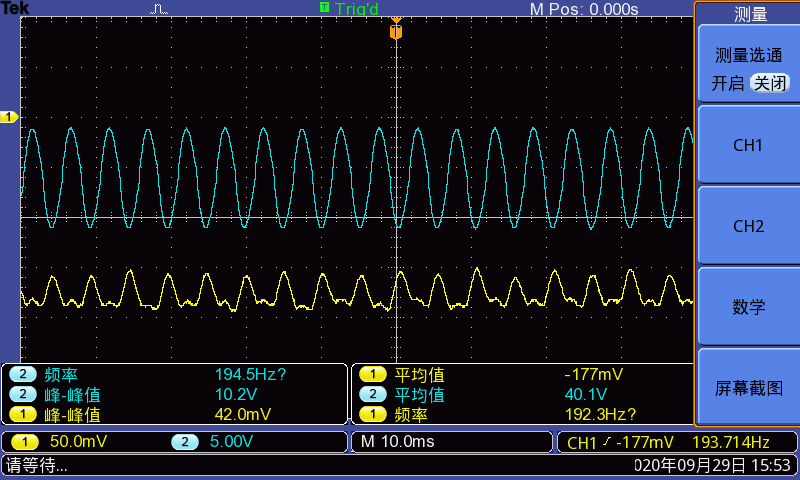
\includegraphics[width=\linewidth]{晶体电光调制图像/没有波片/非线性失真440V/F0000TEK}
    \caption{直流电压440V,下失真}
  \end{subfigure}
  \caption{非线性失真信号的观察}
\end{figure}

之后,调节直流偏压到$484\si{V}$并加入1/4波片不断旋转,转到示波器有特定图像的时候就记录当前波片方向,用光具座上的角度表示。我们发现在角度为250度和270度的时候,图像刚好不失真。

\begin{figure}[H]
  \centering
  \begin{subfigure}{.48\textwidth}
    \centering
    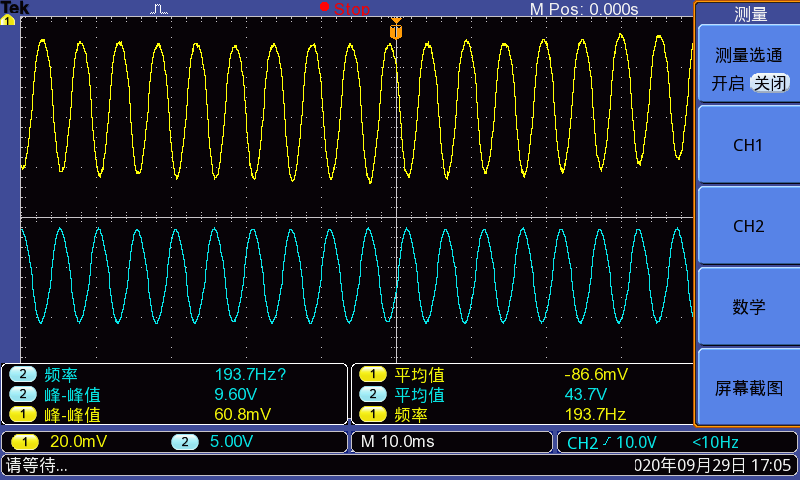
\includegraphics[width=\linewidth]{晶体电光调制图像/有波片/正弦信号484V250度/F0001TEK}
    \caption{偏振片250度,不失真}
  \end{subfigure}
  \begin{subfigure}{.48\textwidth}
    \centering
    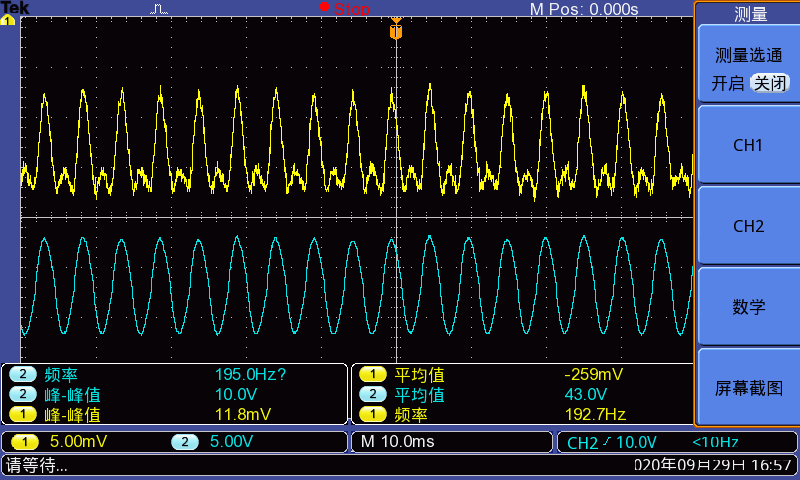
\includegraphics[width=\linewidth]{晶体电光调制图像/有波片/正弦信号478V270度/F0000TEK}
    \caption{偏振片270度,不失真}
  \end{subfigure}
  \caption{加入1/4波片后不失真的信号}
\end{figure}

同时,我们观察到当偏振片的角度为40度和76度时,发生了倍频失真。

\begin{figure}[H]
  \centering
  \begin{subfigure}{.48\textwidth}
    \centering
    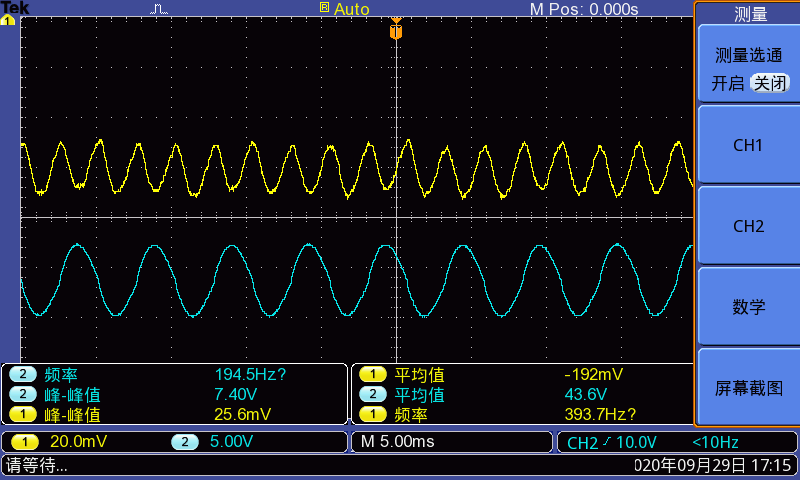
\includegraphics[width=\linewidth]{晶体电光调制图像/有波片/倍频失真484V40度/F0002TEK}
    \caption{偏振片40度,倍频失真}
  \end{subfigure}
  \begin{subfigure}{.48\textwidth}
    \centering
    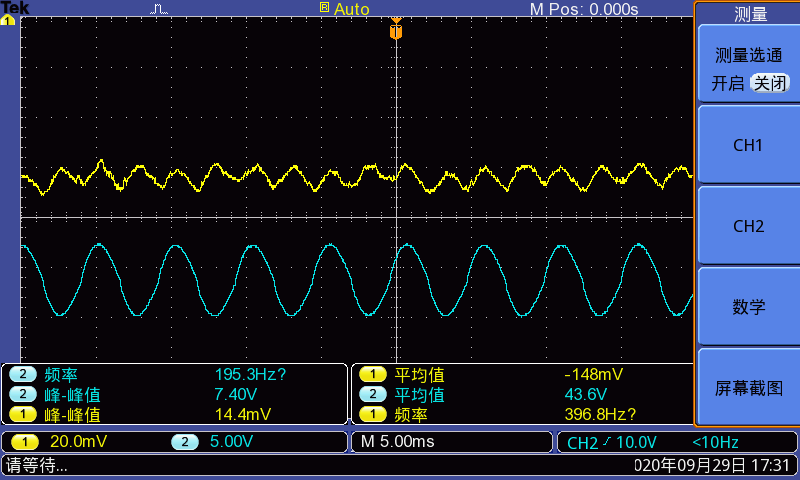
\includegraphics[width=\linewidth]{晶体电光调制图像/有波片/倍频失真484V76度/F0000TEK}
    \caption{偏振片76度,倍频失真}
  \end{subfigure}
  \caption{加入1/4波片后倍频失真的信号}
\end{figure}

而且按照之前的结论,在倍频失真的基础上稍微动波片几度,应当会产生非线性失真。在46度和82度观察到的上失真和下失真证明了这个猜想。

\begin{figure}[H]
  \centering
  \begin{subfigure}{.48\textwidth}
    \centering
    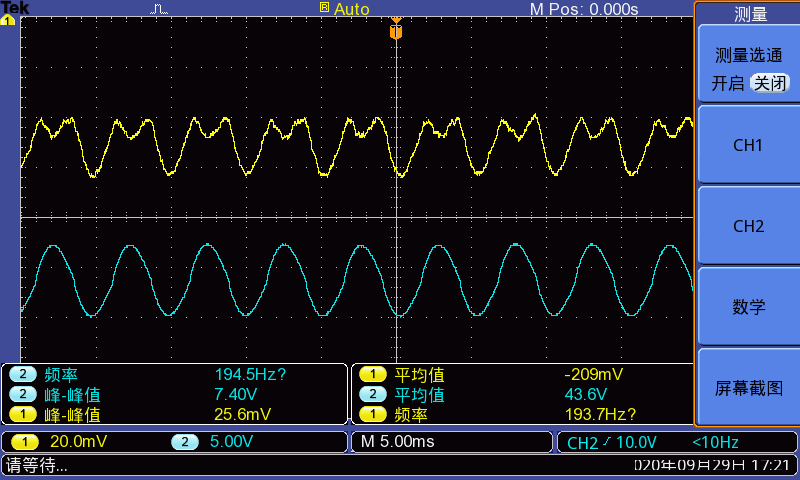
\includegraphics[width=\linewidth]{晶体电光调制图像/有波片/上失真484V46度/F0000TEK}
    \caption{偏振片46度,上失真}
  \end{subfigure}
  \begin{subfigure}{.48\textwidth}
    \centering
    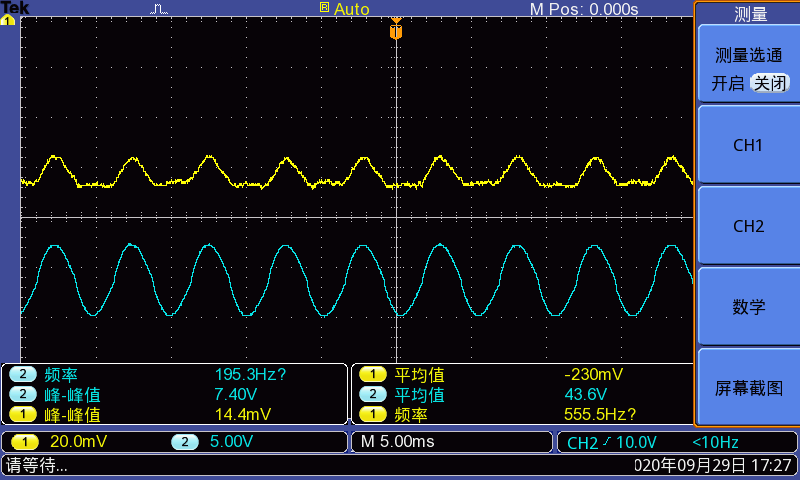
\includegraphics[width=\linewidth]{晶体电光调制图像/有波片/下失真484V82度/F0000TEK}
    \caption{偏振片82度,下失真}
  \end{subfigure}
  \caption{加入1/4波片后非线性失真的信号}
\end{figure}

\subsection{实验中遇到的问题及解决方法}

主要的问题就是偏振片和电光晶体光轴方向不知道的问题,需要想办法让光轴在正确的角度上。解决方法是:把激光器和光强检测装置固定在实验台上,将光强检测装置连接示波器测量电压。放两个偏振片,旋转其中的一个使得示波器显示的电压绝对值为最小值,这时两个偏振片是垂直的。再放入电光晶体,加上电压,此时示波器显示的电压绝对值变大,因为偏振光通过电光晶体发生了旋转,不再和后面的偏振片垂直。此时我们同步转动两个偏振片,保持两个偏振片始终保持垂直,时刻观察示波器显示的电压,达到最小值就停止旋转。这个时候光通过晶体没有发生旋转,电光晶体的两个感应轴是分别和两个偏振片光轴是平行的,再同步旋转两个偏振片45度,两个偏振片和电光晶体的轴就调整好了。

\section{参考文献}
\begin{itemize}[leftmargin=0pt]
  \item[] 近代物理实验讲义
\end{itemize}
\end{document} 
